\documentclass{article}
\usepackage[normalem]{ulem}
\usepackage{amsthm}
\usepackage{mathtools}
\usepackage{thmtools}
\declaretheoremstyle[headfont=\normalfont]{normalhead}
\usepackage{color}
\usepackage{graphicx}
\usepackage{morefloats}
\usepackage{hyperref}
\usepackage{mathrsfs}
\hypersetup{
    colorlinks=false,
    linkcolor=cyan,
    filecolor=cyan,      
    urlcolor=cyan,
}
\usepackage{ amssymb }
\usepackage{textcomp}
\usepackage{mathabx }
\usepackage{url}
\usepackage{float}
\usepackage{biblatex}
\addbibresource{triangle.bib}
\newtheoremstyle{mydef}
{\topsep}{\topsep}%
{}{}%
{\itshape}{}
{\newline}
{%
  \rule{\textwidth}{0.0pt}\\*%
  \thmname{#1}~\thmnumber{#2}\thmnote{\-\ #3}.\\*[-1.5ex]%
  \rule{\textwidth}{0.0pt}}%

\begin{document}
%\theoremstyle{mydef}
\newtheorem{conjecture}{Conjecture}
\newtheorem{theorem}{Theorem}
\newtheorem*{theorem-non}{Theorem}
\newtheorem{remark}{Remark}
\newtheorem{proposal}{Proposal}
\newtheorem{proposition}{Proposition}
\newtheorem*{proposition-non}{Proposition}
\newtheorem{lemma}{Lemma}
\newtheorem{corollary}{Corollary}
\newtheorem{observation}{Observation}
\newtheorem{definition}{Definition}
\newtheorem*{corollary-non}{Corollary}
\author{Barry Brent}

\date{14h 12 May 2021}

\title{Polynomial
interpolation of modular forms for Hecke groups
}
\maketitle
\begin{abstract}
\hskip -.2in
For $m = 3, 4, ...$,
let $\lambda_m = 2 \cos \pi/m$ and
let $J_m (m = 3, 4, ...$) be triangle
functions for the Hecke groups $G(\lambda_m)$
with Fourier
expansions
$
J_m(z) = \sum_{n=-1}^\infty a_n(m)q_m^n,
$
where
$q_m(z) = \exp 2 \pi i z/\lambda_m$.
(When normalized appropriately,
$J_3$ becomes Klein's $j$-invariant
$
j(z) = 1/e^{2 \pi i z} + 744 + ....
$)
For  $n = -1, 0, 1, 2$ and $3$,
Raleigh \cite{raleigh1962fourier}
gave polynomials $P_n(x)$ such that 
$a_{-1}(m)^n q_m^{2n+2} a_n(m) = P_n(m)$
for $m = 3, 4, ...,$
and conjectured that similar 
relations hold for all positive integers
$n$.
Akiyama proved this conjecture in
\cite{akiyama1992note}.
We apply work of Hecke
\cite{berndt2008hecke}
to study experimentally
similar polynomial interpolations
of the $J_m$ Fourier coefficents
and the Fourier coefficients of
other, positive weight, 
modular forms for $G(\lambda_m)$.
We connect these polynomials 
(again, only empirically)
with variants of Dedekind's eta function, 
with the Fourier expansions of some standard
Hauptmoduln, and, in the case of
analogues of Eisenstein series
for $SL(2,\mathbb{Z})$, with certain
divisor sums.
\end{abstract}
\section{Introduction}
Let $\mathbb{Z}, \mathbb{Q}, 
\mathbb{C}$ and $\mathbb{H}$ 
denote, respectively, the set of rational integers,
the set of rational
numbers, the set  of 
complex numbers, and the set of
complex numbers
with positive imaginary parts. 
We write
$\mathbb{H}^* = \mathbb{H} \cup \mathbb{Q} \cup 
\{i \infty\}$, and we equip $\mathbb{H}^*$
with the Poincar{\'e} metric. Figures
$T$ made by three geodesics
of $\mathbb{H}^*$
are called hyperbolic or
circular-arc triangles.
Let $\lambda_m = 2 \cos \pi/m$.
For $m = 3, 4, ...$,
we define the Hecke group
$G(\lambda_m)$
as the discrete group generated by 
the maps $z \rightarrow -1/z$
and $ z \rightarrow z + \lambda_m$.
The full modular group $SL(2,\mathbb{Z})$
is identical to $G(\lambda_3)$.
\newline  \newline \noindent
To define modular forms for
the Hecke groups, we preview
a definition from Berndt  
\cite{berndt2008hecke}, 
which we will quote again
in a later section.
(We depart occasionally from Berndt's
choices of variable to avoid 
clashes with some of our other
notation.)
\newline \newline \noindent
We say that $f$ belongs to the space
$M(\lambda, k, \gamma)$ if
\begin{enumerate}
    \item 
    $$ f(\tau) = \sum_{n = 0}^{\infty}
    a_n e^{2 \pi i n \tau/\lambda},
    $$
    where $\lambda > 0$ and 
    $\tau \in \mathbb{H}$, and
    \item  $f(-1/\tau) = \gamma(\tau/i)^k f(\tau)$,
    where $k > 0$ and $\gamma = \pm 1$.
\end{enumerate}
We say that $f$ belongs to the space
$M_0(\lambda,k, \gamma)$ if $f$ satisfies conditions
1 and 2 and if $a_n = O(n^c)$
for some real number $c$, as $n$ tends to $\infty$.
\newline \newline \noindent
Members of $M(\lambda, k, \gamma)$
are known as modular forms for 
$G(\lambda)$ of weight $k$.
Condition 1 tells us that  they
are invariant under translations
$\tau \mapsto \tau + \lambda$.
Next we preview Berndt's definition
of cusp forms for Hecke groups.
If $f\in M(\lambda, k, \gamma)$
and $f(i \infty) = 0$,
then we call $f$ a cusp form of
weight $k$ and multiplier  $\gamma$
with respect to $G(\lambda)$. 
For cusp forms, the constant terms 
of condition 1 vanish.
We denote by $C(\lambda,k,  \gamma)$ the
vector space of  all cusp forms
of this kind. 
\newline \newline \noindent
For our purposes,
Schwarz triangles $T$ are 
hyperbolic triangles in $\mathbb{H}^*$
with certain restrictions
on the angles at the vertices.
From a Euclidean point of view, 
their sides are
vertical rays, 
segments of vertical rays, 
semicircles 
orthogonal to the real axis
and meeting it
at points $(r,0)$
with $r$ rational,
or arcs of such semicircles.
We choose
$\lambda, \mu$ and $\nu$,
all non-negative, such that
$\lambda + \mu + \nu <1$;
then the angles of $T$
are $\lambda \pi, \mu \pi$,
and $\nu \pi$.
By reflecting $T$ 
across one of its edges, we
get another Schwarz triangle. 
The reflection between
two triangles in $\mathbb{H^*}$
is effected by 
a M\"obius transformation,
so the orbit of $T$
under repeated reflections
is associated to a 
 collection of 
 M\"obius transformations.
The group 
 generated by 
these transformations is a
triangle group.
By the Riemann Mapping Theorem
there is a conformal, onto 
map
$\phi: T \mapsto \mathbb{H}^*$
called a triangle function.
\newline \newline \noindent
Hecke groups 
\cite{hecke1936bestimmung}
are triangle groups 
$H$ that act 
properly discontinuously 
on $\mathbb{H}$.
This means that for compact 
$K \subset \mathbb{H}$, the set
$\{\mu \in H$ s.t. \hskip -.05in
$K \cap \mu(K) \neq \emptyset\}$
is finite.
Recall that 
$G(\lambda_m)$ is the Hecke group
generated by the maps 
$\tau \mapsto -1/\tau$
and $\tau \mapsto \tau + \lambda_m$.
Apparently 
it was Hecke who, 
also in \cite{hecke1936bestimmung},
established that 
$G(\lambda_m)$ has the structure
of a free product 
of cyclic groups
$C_2 * C_m$,
generalizing the relation
\cite{serre1970course, cangul1996group}
$SL(2,\mathbb{Z}) = C_2 * C_3$.
\newline \newline \noindent
Let $\rho = -\exp(-\pi i/m) = 
-\cos(\pi/m) + i\sin(\pi/m)$, and
let $T_m \subset \mathbb{H}^*$ 
denote the 
hyperbolic triangle with vertices
$\rho, i$, and $i\infty$. 
The corresponding angles are 
$\pi/m, \pi/2$ and $0$
respectively. Let 
$\phi_{\lambda_m}$ be a 
triangle function 
for $T_m$. The
function $\phi_{\lambda_m}$ 
has a pole at $i\infty$
and period $\lambda_m$.
For $P, Q \in \mathbb{H}^*$,
let us us write $P \equiv_H Q$ when 
$\mu \in H$ and $Q = \mu(P)$.
Then $\phi_{\lambda_m}$ extends to 
a function
$J_m: \mathbb{H}^* \rightarrow \mathbb{H}^*$ by
declaring that
$J_m(P) = J_m(Q)$
if and only if 
$P \equiv_H Q$.
$J_m$ is a modular function
for $G(\lambda_m)$.
\newline \newline \noindent
Schwarz \cite{schwarz1873ueber}, 
Lehner \cite{lehner1954note},
Raleigh \cite{raleigh1962fourier}
and others
studied Schwarz triangle functions, 
which map  hyperbolic triangles $T$ in the 
 extended upper half $z$-plane  onto
 the extended upper half $w$-plane.
 For certain $T = T_m$, 
a triangle function 
$\phi_{\lambda_m}: T \to \mathbb{H}^*$
 extends to a map
$J_m: \mathbb{H}^* \rightarrow \mathbb{H}^*$
 invariant under
modular transformations
from $G(\lambda_m)$.
Suitably normalized, the $J_m$
become analogues 
$j_m$ of the normalized
Klein's modular invariant 
$$
j(z) = -1/q + 744 + 196884 q + ...
$$
where $q = q(z) = \exp (2 \pi i z)$ 
 and $j_3(z) = j(z)$.
 \newline \newline \noindent
With $\lambda_m = 2 \cos \pi/m$ and 
$q_m(z) = \exp (2 \pi i z/\lambda_m)$,
the original $J_m$ have Fourier series
$J_m(z)= \sum_{n \geq -1} a_n(m) q_m(z)^n$.
For  $n = -1, 0, 1, 2$ and $3$,
Raleigh \cite{raleigh1962fourier}
gave polynomials $P_n(x)$ such that 
$a_{-1}(m)^n q_m^{2n+2} a_n(m) = P_n(m)$
for $m = 3, 4, ...,$
and conjectured that similar 
relations hold for all positive integers
$n$.
Akiyama \cite{akiyama1992note}
proved Raleigh's conjecture
 in the passage 
after his (Akiyama's) equation (6).
\newline  \newline \noindent Hecke 
(\cite{berndt2008hecke}, \cite{hecke1936bestimmung})
built families of modular forms $f_m$
 for $G(\lambda_m)$
sharing particular properties,
such as their weight;
we will describe his construction later.
Earlier authors, whose work we will 
also describe,
had already built modular functions
(meromorphic functions
invariant under the
action of $G(\lambda)$,
thus, of weight zero)
from triangle functions.
\newline \newline \noindent
The plan of the article is as follows.
We sketch 
the theory of Schwartz triangles; then,
the construction of their
triangle functions;
from the triangle functions,
the modular functions
for the Hecke groups;
and, from them,
 modular forms
for these groups.
To this point,
the article is just
a summary of
background
material.
By methods familiar
from the classical case, 
we then construct modular forms
with rational Fourier expansions,
describe our modifications of them,
and describe computer experiments
on the modifications. 
\footnote{We documented our experiments in
a series of \it Mathematica \rm notebooks
and accompanying data files.
That material 
is in a \it Github \rm repository 
named ``interpolations'' \cite{test3}. 
A green ``Code'' button on the top page of 
the repository contains a drop-down menu
with a download option.
We tried to
make the remarks, clauses
of conjectures, \it etc., \rm findable by
reading the file names. Data files
(in plain text format) 
are named less transparently, but
they are defined within the
documents where they were generated.
A \it Mathematica \rm notebook 
(``mf23.nb'') in the repository
contains a searchable library 
of functions that may not be defined
explicitly within notebooks 
containing code that calls them.}
\newline \newline \noindent
The experiments indicate that the Fourier
expansions of several
Hecke modular forms are interpolated
in the sense of Raleigh by polynomials.
We describe connections among
these polynomials, certain
divisor sums, and Hauptmoduln 
discussed in  the
Moonshine literature.
We offer only conjectures; 
we prove no theorems
of our own. All theorems that
we mention are part of
the existing literature.
\newline \newline \noindent
The earliest 
computer code
we located 
for calculating 
Fourier 
expansions of 
triangle functions for Hecke groups
is that of Leo; 
it is based on Lehner's 
construction. Leo also
calculates the Fourier coefficients
of weight 4 and weight 6
Hecke-analogues of classical Eisenstein
series in Chapter 4 of \cite{leo2008fourier}.
Our code for triangle functions,
which is based on Leo's,
comes from the papers of 
Lehner and Raleigh.
J. Jermann's package \cite{sagemath}
is also concerned with modular forms
of triangle groups for Hecke groups,
but we did not use his code in our experiments.
For definiteness, we transcribe
our code defining triangle functions
and modular forms in an appendix.
\section{A glossary}
Several special functions in this list 
are so closely related that one might
wish to know why we have included all of them.
It is for the convenience of both
the reader and ourselves, because
differing forms (basically
just different notations)
are used by Lehner and Raleigh, 
and we hope in this way to discuss
both of them while avoiding confusion.
\begin{enumerate}
\item The digamma function
$\psi(z):=\Gamma'(z)/\Gamma(z)$.
\item The Schwarzian derivative
(\cite{caratheodory2}, p. 130, 
equation 370.8)
\begin{equation}
\{w,z\} = 
\frac{2 w' w''' - 3w''^2}{2w'^2}
\end{equation}
for $w = w(z)$.
\item The Pochhammer  symbol
$$
(a)^0: = 1 \text{ and, for }
n \geq 1,
(a)^n:=a(a+1)...(a+n-1) = \Gamma(a+n)/\Gamma(a).
$$
\item The function $c_{\nu}$ given by (\cite{caratheodory2}, 
p. 138, equation 377.3)
$$
c_{\nu} = c_{\nu}(\alpha, \beta, \gamma) :=  
\frac{(\alpha)^{\nu} (\beta)^{\nu}}
{{\nu}!(\gamma)^{\nu}}, {\nu} \geq 0.
$$
To facilitate comparison with
Raleigh's  
equation ($9^1$) 
\cite{raleigh1962fourier}, we remark that 
\begin{equation}
c_{\nu} = 
\frac{\Gamma(\alpha + {\nu})}{\Gamma(\alpha)}
\cdot \frac{\Gamma(\beta + {\nu})}{\Gamma(\beta)}
\cdot \frac{\Gamma(1)}{\Gamma(1 + {\nu})}
\cdot \frac{\Gamma(\gamma)}{\Gamma(\gamma + {\nu})}.
\end{equation}
In the terms of this article's Theorem 1 
below, Raleigh is treating the
case $\lambda = 0$, for which 
(equation (6) below) $\gamma = 1$
and the expression on the right side of (2)
becomes, as in Raleigh,
$$\frac{\Gamma(\alpha + {\nu})\Gamma(\beta + {\nu})}
{\Gamma(\alpha)\Gamma(\beta)({\nu}!)^2}.$$
\item The function $e_{\nu}$ given by
(\cite{raleigh1962fourier}, equation $9^1$)
$$
e_{\nu} = e_{\nu}(\alpha, \beta) :=  
\sum_{p = 0}^{{\nu} - 1}
\left ( \frac 1{\alpha + p} + 
\frac 1{\beta + p} 
- \frac 2{1 + p} \right ).
$$
Here, we are dealing with the 
same ambiguity present in the
definition of $c_{\nu}$:
this is a specialization to the
case $\gamma = 1$ of the
$e_{\nu}$ 
for ${\nu} \geq 1$
given by (\cite{caratheodory2}, p. 153,
equation 387.5)
$$
e_{\nu} = e_{\nu}(\alpha, \beta, \gamma) :=  
\sum_{p = 0}^{n - 1}
\left ( \frac 1{\alpha + p} + 
\frac 1{\beta + p} 
- \frac 2{\gamma + p} \right ).
$$ Unless it
is explicitly indicated to be
otherwise, we intend the former (Raleigh's)
definition.
\item 
\begin{enumerate}
    \item Gauss's hypergeometric series
given by \cite{caratheodory2}, p. 138,
equation (377.4),
$$
F(\alpha,\beta,\gamma;\tau):=
\sum_{{\nu}=0}^{\infty} 
c_{\nu}(\alpha, \beta, \gamma) \tau^{\nu}$$
$F$ is occasionally written in 
\cite{caratheodory2} as $\phi_1$ (for
example, on, p. 152.)
    \item As
    defined in the first line of
\cite{caratheodory2}, p. 142:
$$
F_1(\alpha,\beta,\gamma; \tau):=
F(\alpha,\beta,\gamma+1;\tau).
$$

    \item Alternatively,
    dropping $\gamma$, as defined in 
    \cite{leo2008fourier}, equation (3.5):
$$
F_1(\alpha,\beta;z):= 
\sum_{\nu=1}^{\infty}
\frac{(\alpha)_k(\beta)_{\nu}}{(\nu!)^2}
e_{\nu}(\alpha, \beta).$$
It is in the latter form, defined
more cryptically in \cite{lehner1954note}, p. 244,
that we will use $F_1$; to
establish his series for the triangle functions,
which we will apply below,
Lehner uses this definition of
$F_1$, as well as certain 
theorems from  Fricke
\cite{fricke1922elliptischen}.
Referring to item 4, we see that
$$
F_1(\alpha,\beta;z)= 
\sum_{\nu=1}^{\infty}
c_{\nu}(\alpha,\beta,1)
e_{\nu}(\alpha, \beta).$$
We will derive another form of $F_1(\alpha,\beta;z)$
in item 7.
\end{enumerate}
\item With 
$F = F(\alpha, \beta, \gamma;\tau)$,  
a special function
$$F^*(\alpha, \beta, \gamma;\tau): = 
\frac{\partial F}{\partial \alpha} + 
\frac{\partial F}{\partial \beta}+ 
2\frac{\partial F}{\partial \gamma};$$
by \cite{caratheodory2}, equation (387.4) on p. 153, 
$F^*$ may be written
$$
F^*(\alpha, \beta, \gamma;\tau) =
\sum_{{\nu} = 1}^{\infty}
c_{\nu} (\alpha, \beta, \gamma) 
e_{\nu} (\alpha, \beta, \gamma) \tau^{\nu}.
$$
It follows that $F^*(\alpha, \beta, 1;\tau) = F_1(\alpha,\beta;z)$.
\item A special  function
$\phi_2^*(\tau)$ is defined as a certain limit
(\cite{caratheodory2},
p. 152, equation 386.2)
but is immediately (equation 386.3) 
reduced to 
$$\phi_2^*(\tau) =  
F(\alpha, \beta, 1;\tau) \log \tau
+ F^*(\alpha, \beta, 1;\tau).$$
\item The set $\mathscr{Q} 
=\{2,5,6,8,10,11,14,15,17,18,20,22,23,...\}$
of positive integers not
represented by the quadratic form
$x^2+xy+y^2$ \cite{OEIS}. B. Cloitre
asserts, on the same O.E.I.S.
page, that  $\mathscr{Q}$ is also the set of
non-negative integers $n$
such that
$\delta(n)$ is non-zero, where
$\eta$ is Dedekind's eta function and
$\sum_n \delta(n)x^n = \eta(x^3)/\eta(x)^3.$
\item The McKay-Thompson series of class 4A,
$\{1,24, 276, 2048, ...\}$, which is
the sequence of coefficients 
in the $q$-series of a certain
hauptmodul discussed in \cite{doi}.
McKay relates
the hauptmoduln treated in that paper 
to Dedekind's eta function.
We identified the class 4A
McKay Thompson series with the
$\overline{a}_n$ of our
conjecture 1 after finding it 
in the \it On-line Encyclopedia
of Integer Sequnces \rm \cite{OEIS2}.
\end{enumerate}
\section{Calculation of Schwarz's inverse 
triangle function}
Schwarz
proved 
\begin{theorem}
 (\cite{caratheodory2}, \textsection 374)
\begin{enumerate}
\item
Let the half-plane $\Im z > 0$ be mapped
conformally onto an arbitrary 
circular-arc triangle
whose angles at its vertices $A, B$, and $C$ 
are $\pi \lambda, \pi \mu$, and $\pi \nu$, and
let the vertices $A, B, C$ be the images of
the  points $z = 0, 1, \infty$, respectively.
Then the mapping function $w(z)$ must be 
a solution of the third-order differential
equation
\begin{equation}
\{w,z\} =
\frac{1-\lambda^2}{2 z^2} +
\frac{1-\mu^2}{2(1-z^2)} +
\frac{1-\lambda^2-\mu^2+\nu^2}
{2z(1-z)}.
\end{equation}
\item
If $w_0(z)$ is any solution
of equation (3) that satisfies
$w'_0(z) \neq 0$ at all interior points
of the half-plane, then the function
$$
w(z) = \frac {aw_0(z) + b}{cw_0(z) + d}
\hskip 1in (ad - bc \neq 0)
$$
is likewise a solution of equation 3.
\item
Also, every solution of equation (3) that is regular
and non-constant in the half-plane $\Im z > 0$
represents a mapping of this half-plane onto a
circular-arc triangle with angles $\pi \lambda,
\pi \mu,$ and $\pi \nu$.
\end{enumerate}
\end{theorem}
\noindent
In Carath{\'e}odory's lexicon
(\cite{caratheodory1} p. 124),
a regular function is one that is
differentiable 
on an open connected set.
Carath{\'e}odory writes the left side
of (3) as 
``$\{w,z\} = \frac{w^{'}w^{'''} - 
3 w^{''2}}{w^{'2}} = ...$'', 
but this is not the case.
We infer that the Schwarzian derivitave $\{w,z\}$ 
is intended
from the automorphy property of clause 2.
\newline \newline \noindent
Let us write
\begin{equation}
\alpha = \frac 12
(1 - \lambda - \mu + \nu),
\end{equation}
\begin{equation}
\beta = \frac 12(1-\lambda - \mu - \nu),
\end{equation}
and
\begin{equation}
\gamma = 1 - \lambda.
\end{equation}
The solutions $w$ of (3)
are inverse to triangle functions;
they are quotients of 
arbitrary solutions of
\begin{equation}
u'' + p(z)u' +q(z)u = 0
\end{equation}
when (\cite{caratheodory2}, 
p. 136, equation (376.4))
 $$
 p = \frac {1-\lambda}z-\frac {1-\mu}{1-z}
 $$
 and
 $$
 q = - \frac {\alpha \beta}{z(1-z)}.
 $$
Equation (7) reduces (\cite{caratheodory2}, p. 137, 
equations 376.5-7)
to the 
hypergeometric differential
equation 
\begin{equation}
z(1-z)u'' +(\gamma - (\alpha + \beta +1)z)u'
- \alpha \beta u = 0.
\end{equation}
As long as $\gamma$ is not a
non-positive integer, 
$u=F(\alpha,\beta,\gamma;z)$
is a solution of (8); it is 
the only solution
regular at $z = 0$, and it
satisfies 
$F(\alpha,\beta,\gamma;0) = 1$
(final paragraph of 
\cite{caratheodory2}, \textsection 377, 
p. 138.) 
 \newline \newline \noindent
 In  \cite{caratheodory2},
\textsection \textsection 386-388 
(pp. 151-155), we find that
when $\gamma = 1$
and $\lambda = 0$,
 another, linearly independent,
solution of equation (7) is $\phi_2^*(z)$.
\cite{caratheodory2}, Section 394, pp. 165 - 167 
 is 
devoted to the
case $\lambda = 0$. 
The mapping 
function $w$ of Theorem 1 
satisfies (\cite{caratheodory2}, 
p. 166,  equation 394.4)
\begin{equation}
 w = \frac 1{\pi i}
 \left [ \frac{\phi_2^*}{\phi_1} -
\left (2 \psi(1) - 
\psi(1 - \alpha)
- \psi(1-\beta) \right ) \right ] + 
i \frac{ \sin \pi \mu}
{\cos \pi \mu + \cos \pi \nu}.
\end{equation}
\section[]{Inversion of Schwarz's 
inverse triangle function}
Following Lehner and Raleigh,
we consider the Schwarz triangle
$T_m$ with vertices at 
$\rho = -\exp(-\pi i/m), i$,
and $i\infty$. 
In terms of
Theorem 1,
$T_m$ has
$\lambda = 0$
(an angle $0$ at 
the vertex $i\infty$), $\mu = 1/2$
(an angle $\pi/2$ at $i$),
and $\nu = 1/m$ (an angle $\pi/m$
at $\rho$.)
 In this situation, $\gamma = 1$. 
 \newline \newline \noindent
 Let $J_m$ be automorphic for 
 $G(\lambda_m)$ with
 $J_m(\rho) = 0, J_m(i) = 1$,
 and $J_m(i \infty) = \infty$.
 In terms of Theorem 1, $w$
 and $J_m$ are inverse functions.
 We are going to write
 down the Fourier expansion
 $\sum_{n = -1}^{\infty} a_n q_m(z)^n$
 of $J_m$.
 \newline \newline \noindent
By clause 2 of Theorem 1, if $w$ satisfies 
equations (3) and (9), so does
$\tau = \thinspace \tau(z) = \lambda_m w(z)/2$, 
and therefore
$$
2\pi i\tau /\lambda_m =
 \frac{\phi_2^*}{\phi_1} - \left (2 \psi(1) - 
\psi(1 - \alpha)
- \psi(1-\beta) \right ) - 
\pi  \sec(\pi/m).
$$
Let us write
$\log A_m = -2 \psi(1) + \psi(1 - \alpha)
+ \psi(1 - \beta)  - \pi \sec(\pi/m).$ 
In general, $A_m = a_{-1}(m)$
(\cite{raleigh1962fourier},
for example two lines below equation (12).)
Recalling the definitions of 
$\phi_1$ and $\phi_2^*$
from our glossary items 6 and 8, 
we find (abbreviating $J_m(\tau)$ as $J_m$) that 
\begin{equation}
2\pi i\tau /\lambda_m 
  = - \log J_m
+ \frac {F^*(\alpha, \beta, 1;1/J_m)}
{F(\alpha, \beta, 1;1/J_m)} +  
\log A_m.
\end{equation}
Equation (10) is equation (6) of 
\cite{raleigh1962fourier},
but Raleigh  suppresses the 
subscripts.
He also writes 
$\exp 2 \pi i \tau/\lambda_m$ as $x_m$, 
so that (in our earlier notation)
$x_m = q_{_m}(\tau)$.
\newline \newline \noindent
In Raleigh's notation, after taking
exponentials,
\begin{equation}
 x_m/A_m = 
\frac 1{J_m} \exp 
\frac {F^*(\alpha, \beta, 1;1/J_m)}
{F(\alpha, \beta, 1;1/J_m)},
\end{equation}
the right side of
which has a power series in $J_m$ with
rational coefficients. 
Writing $X_m = x_m/A_m$
we can regard $X_m = X_m(J_m)$ as a power series
in $J_m$.
Following \cite{lehner1954note} and
 \cite{raleigh1962fourier},
we inverted this power series to obtain
one for the modular function $J_m$.
Let $\mathscr{I}$
be a formal operation
taking a power series $\sigma(v)$
to its inverse; that is,
if $u=\sigma(v)$ then 
$v = \mathscr{I}(\sigma)(u)$.
Let  $Y_m(J)$ be a power series
such that
$$ Y_m(J_m) = J_m \exp 
\frac {F^*(\alpha, \beta, 1;J_m)}
{F(\alpha, \beta, 1;J_m)} = 
X_m \left (1/J_m \right )$$
and hence
$$
Y_m(1/J_m) =
\frac 1{J_m} \exp _m
\frac {F^*(\alpha, \beta, 1;1/J_m)}
{F(\alpha, \beta, 1;1/J_m)} = X_m(J_m),$$
so that $\mathscr{I}(Y_m)(X_m(J)) = 1/J_m$
and, therefore,
 $J_m = 1/\mathscr{I}(Y_m)(X_m)$.
 \newline \newline \noindent
We noticed several typos in
\cite{raleigh1962fourier}.
Four of Raleigh's equations---(I), (10), and
the two equations on p. 109
that begin ``$a_{-1}(q) = ...$''
(where his $q$ is our $m$)---are 
pairwise contradictory.
From the second paragraph
on Raleigh's p. 110, we expect that 
$A_3 = a_{-1}(3) = 1/1728, A_4 = a_{-1}(4) = 1/256$, and 
$A_6 = a_{-1}(6) = 1/108$. These values
are consistent with Raleigh's equation 
(10), but not with the others.
We infer that all of them except (10) are incorrect.
Thus, following Raleigh by
writing  $\psi$ for the digamma function,
$\alpha(m)$ for $(1/2-1/m)/2$, and 
$\beta(m)$ for $(1/2+1/m)/2$, 
\begin{equation}
a_{-1}(m) = \exp\left (-2 \psi(1) + \psi(1-\alpha(m))
+\psi(1 - \beta(m))- \pi \sec(\pi/m)
\right ).
\end{equation}
\section{Modular forms 
from modular functions}
When the  
$w$-image of $\mathbb{H}^*$ is
$T_m$, the inverse of $w$ is
$\phi_{\lambda_m}$. 
$J_m$, the extension 
by modularity of $\phi_{\lambda_m}$ to
$\mathbb{H}^*$, is periodic
with period $\lambda_m$ and
maps $\rho$ to $0$, $i$ to $1$, 
and $i\infty$ to $\infty$
(\cite{lehner1954note},
equation (2).)
These mapping properties
allow us, following Berndt's exposition
\cite{berndt2008hecke}
of Hecke,
to construct positive 
weight modular forms for $G(\lambda_m)$
from $J_m$.
This section describes results of Hecke
that are perhaps most easily accessible
for the classical case $m = 3$ 
in Schoeneberg
\cite{schoeneberg1974} and, 
for the general case, in 
 Berndt  \cite{berndt2008hecke}.
\subsection[]{The case $m=3$.}
By keeping
track
of the weights, zeros and poles of the
constituent factors in the 
numerator and denominator of the
fraction defining
$$ f_{a,b,c} = 
\frac{J^{'a}}
{J^b (J - 1)^c},
$$
Schoeneberg \cite{schoeneberg1974} 
(Theorem 16, p.45)
demonstrates  that $f_{a,b,c}$
is an entire modular form of weight $2a$
for $SL(2,\mathbb{Z})$
 if $a \geq 2, 3c  \leq a, 3b \leq 2a$,  
 $b+c \geq a$ and $a, b, c$ are integers.
(Schoeneberg speaks of ``dimension $-2a$.'')
Thus he is able to 
write down a weight $4$ entire modular form
$E^*_4 = f_{2,1,1}$
for $SL(2,\mathbb{Z})$ with a zero
of order $\frac 13$ at $\rho = e^{2 \pi i/3}$
and a weight $6$ 
entire modular form 
$E^*_6 = f_{3,2,1}$
for $SL(2,\mathbb{Z})$
with a zero of order $\frac 12$
at $i$.
(Schoeneberg writes $G^*_4, G^*_6$.)
It is well known that the 
(vector space) dimension of the
spaces of weight $4$ and $6$ entire
modular forms for $SL(2,\mathbb{Z})$
is equal to one,
so $E^*_4$ and  $E^*_6$ 
may be identified
with the usual weight $4$ 
and weight $6$ 
Eisenstein series,
up to a  normalization. 
Finally, Schoeneberg defines
the weight $12$ cusp form
$\Delta^* = E_4^{*3} - E_6^{*2}$
with a zero of order $1$ at $i \infty$. 
It is a multiple of $\Delta$.
\subsection[]{The case $m \geq 3$.}
We quote statements from Berndt  
\cite{berndt2008hecke}, which is
an exposition of Hecke's 
\cite{hecke1938lectures} and
other writings. 
We depart occasionally from Berndt's
choices of variable to avoid 
clashes with our earlier
notation.
\begin{definition}
(\cite{berndt2008hecke}, Definition 2.2)
We say that $f$ belongs to the space
$M(\lambda, k, \gamma)$ if
\begin{enumerate}
    \item 
    $$ f(\tau) = \sum_{n = 0}^{\infty}
    a_n e^{2 \pi i n \tau/\lambda},
    $$
    where $\lambda > 0$ and 
    $\tau \in \mathbb{H}$, and
    \item  $f(-1/\tau) = \gamma \cdot (\tau/i)^k f(\tau)$,
    where $k > 0$ and $\gamma = \pm 1$.
\end{enumerate}
We say that $f$ belongs to the space
$M_0(\lambda,k, \gamma)$ if $f$ satisfies conditions
1 and 2, and if $a_n = O(n^c)$
for some real number $c$, as $n$ tends to $\infty$.
\end{definition}
\noindent
After defining the notion of a fundamental 
region in the usual
way and defining as $G(\lambda)$ the group 
of linear fractional transformations
generated by
$\tau \mapsto -1/\tau$ and
$\tau \mapsto \tau + \lambda$,
Berndt states (for $\tau = x + iy$)
\begin{theorem}
(\cite{berndt2008hecke}, Theorem 3.1)
Let $B(\lambda)= \{\tau \in \mathbb{H}:
x < \lambda/2,  |\tau| > 1\}$. Then if 
$\lambda \geq 2$ or if $\lambda = 2 \cos(\pi/m)$,
where $m \geq 3$ is an integer, $B(\lambda)$ is
a fundamental region for $G(\lambda)$.
\end{theorem}
\begin{definition}
(\cite{berndt2008hecke}, Definition 3.4)
Let $T_A = \{ \lambda: 
\lambda = 2 \cos(\pi/m), m \geq 3, m \in \mathbb{Z}\}$.
\end{definition}
\noindent
Berndt states in his Theorem 5.4 that 
$G(\lambda)$ is discrete if and only if
$\lambda$ belongs to $T_A$. This discreteness
is the premise of the theory of 
automorphic functions generally.
He embeds within the
proof of his Lemma 3.1 
(which we omit), the 
\begin{definition}
$\tau_{\lambda}$ denotes the intersection
in $\mathbb{H}$ of the line
$x = -\lambda/2$ and the unit circle
$|\tau| = 1$. 
\end{definition} \noindent
(Berndt remarks at the top of page 35 that
$\tau_{\lambda}$ is the lower left corner
of $B(\lambda)$). and that
$\pi \theta = \pi - \arg(\tau_{\lambda})$,
so that $\cos (\pi \theta) = \lambda/2$.)
\newline \newline \noindent
To characterize Eisenstein series,
we need to keep track of some analytical
properties. The next definition summarizes
the second paragraph  of
Berndt's Chapter 5.
(Throughout his Chapter 5, $\lambda < 2$.)
\begin{definition}
Let $f \in M(\lambda, k, \gamma), f$
not identically zero.
    \begin{enumerate}
    \item
    $N = N_f$ counts the zeros of $f$ on 
    $\overline{B(\lambda)}$  with multiplicities.
    \item $N_f$ does not count zeros
    at $\tau_{\lambda}$, at $\tau_{\lambda} + \lambda$, 
    at $i$, or at $i\infty$.
    \item 
    If $\tau_0 \in 
    \overline{B(\lambda)}, f(\tau_0) = 0$
    and
   $\Re (\tau_0) = -\lambda/2$, 
    then $f(\tau_0 + \lambda) = 0$ and
    $N_f$ counts only one of the two zeros.
    \item If $\tau_0 \in 
    \overline{B(\lambda)}, f(\tau_0) = 0$,
    and $|\tau_0| = 1$, then,
     $f(-1/\tau_0) = 0$,
    and $N_f$ counts only one 
    of these two zeros.
    \item  The numbers $n_{\lambda}, n_i,$
    and $n_{\infty}$ are the orders of the
    zeros of $f$ at $\tau_{\lambda},
    i$ and $i\infty$, repectively.
    The order $n_{\infty}$ is measured in terms of
    $\exp(2 \pi i \tau/\lambda)$.
\end{enumerate}
\end{definition}
\noindent
The multiplier $\gamma$ is given by
\begin{theorem}
(\cite{berndt2008hecke}, Corollary 5.2)
Let $f \in M(\lambda,k,\gamma)$ and 
let $n_i$ be the order of the zero
of $f$ at $\tau = i$.
Then
$$
\gamma= (-1)^{n_i}.
$$
\end{theorem}
\noindent
The next two results 
tell us that the only nontrivial
case in this theory is the one 
that we are interested in.
\begin{theorem} 
(\cite{berndt2008hecke}, Lemma 5.1)
If $\dim M(\lambda,k,\gamma)
\neq 0$,
$$
N_f + n_{\infty} + \frac 12 n_i + 
\frac {n_{\lambda}}m =
\frac 12 k \left ( \frac 12 - \theta \right).
$$
\end{theorem}
\noindent
By Berndt's equation (5.16), 
if $m \geq 3$ then 
the right side can be written as $k(m-2)/4m$.
\begin{theorem}
(\cite{berndt2008hecke}, Theorem 5.2)
If $\dim M(\lambda,k,\gamma)
\neq 0$, then $\theta = 1/m$
where $m \geq 3$ and $m \in \mathbb{Z}$.
\end{theorem}
\noindent
We are concerned with
 $\lambda \in T_A$. 
This makes $\lambda < 2$ as in all 
the results of Berndt's 
Chapter 5.
\newline \newline \noindent
One estimate 
for $\dim M(\lambda, k, \gamma)$ is 
\begin{theorem}
(\cite{berndt2008hecke}, Theorem 5.6)
If $\lambda \notin T_A$, then
$\dim M(\lambda,k,\gamma) = 0$.
If $\lambda = 2\cos(\pi/m) \in T_A$,
then for nontrivial $f \in
M(\lambda,k,\gamma)$, the weight
$k$ has the form
$$
k = \frac {4h}{m-2} + 1 - \gamma,
$$
where $h \geq 1$ is an integer.
Furthermore,
$$
\dim M(\lambda,k,\gamma) = 1 + \left \lfloor
\frac{h + (\gamma-1)/2}m \right \rfloor.
$$
\end{theorem}
\noindent
Eliminating $h$, we find that
\begin{equation}
\dim M(\lambda,k,\gamma) = 1 +
\left \lfloor 
k\left (\frac 14 - \frac 1{2m} \right ) + 
\frac {\gamma}4 - 
\frac 14
\right \rfloor.
\end{equation}
Berndt  (\cite{berndt2008hecke}, Remark 5.3)
proves that the  dimension formula 
 above holds also
 when $h = 0$.
 \newline  \newline \noindent
The existence of 
 certain modular forms is
 provided by
 \begin{theorem}
 (\cite{berndt2008hecke}, Theorem 5.5)
 Let $\lambda \in T_A$. Then there exist
 functions $f_{\lambda}, f_i$, and 
 $f_{\infty} \in M(\lambda,k,\gamma)$
 such that each has a simple zero at 
 $\tau_{\lambda}, i$, and $i \infty$,
 respectively, and no other zeros. 
 Here, $\gamma$ is given by 
 [Theorem 3 (this article)],
 and $k$ is determined in each case from
 [Theorem 4 (this article)].
 Thus, $f_{\lambda} \in 
 M(\lambda, 4/(m-2), 1), f_i \in 
 M(\lambda, 2m/(m-2), -1)$, and
 $f_{\infty} \in M(\lambda, 4m/(m-2),1)$.
 \end{theorem}
 \begin{remark}
 (\cite{berndt2008hecke}, pages 47-48)
By the Riemann mapping theorem
there exists a function $g(\tau)$ that
maps the simply connected region $B(\lambda)$
one-to-one and conformally
onto $\mathbb{H}$. If
we require that
$g(\tau_{\lambda}) = 0,
g(i) = 1$, and $g(i\infty) = 
\infty$, then $g$ is determined uniquely.
 \end{remark}
 \noindent
 Now we can write down 
 $f_{\lambda}, f_i$, and $f_{\infty}$ explicitly.
 The next theorem is extracted from 
the proof of Theorem 7.
$f_{\lambda}$ and $f_i$
correspond to Eisenstein series and 
$f_{\infty}$ to a cusp form.
In our code, we take
 $g$ to be a normalized form of $J_m$.
 \begin{theorem}
 (\cite{berndt2008hecke}, page 50)
 $$
 f_{\lambda}(\tau)
 =\left \{
 \frac {g'(\tau)^2}
 {g(\tau)(g(\tau) -1)}
 \right \}^{1/(m-2)},
 $$
 $$
 f_i(\tau) =
 \left \{
 \frac {g'(\tau)^m}
 {g(\tau)^{m-1} (g(\tau) - 1)}
 \right \}^{1/(m-2)},
 $$
 and
 $$
 f_{\infty}(\tau) = 
 \left \{ \frac{g'(\tau)^{2m}}
 {g(\tau)^{2m-2}(g(\tau)-1)^m}
\right \}^{1/(m-2)}.
 $$
 \end{theorem}
 \noindent
In our applications to Lehmer's
problem, we will be
interested in the dimensions
of the weight $12$ cusp spaces
for $\lambda = \lambda_m = 2 \cos \pi/m$.
\begin{definition}
(\cite{berndt2008hecke}, Definition 5.2)
If $f\in M(\lambda, k, \gamma)$
and $f(i \infty) = 0$,
then we call $f$ a cusp form of
weight $k$ and multiplier  $\gamma$
with respect to $G(\lambda)$. 
We denote by $C(\lambda,k,  \gamma)$ the
vector space of  all cusp forms
of this kind.
\end{definition}
\begin{remark}
(\cite{berndt2008hecke}, equation (5.25))
$$\dim C(\lambda, k,  \gamma) \geq 
\dim M(\lambda, k,  \gamma) -1.$$
\end{remark}
\begin{remark}
In view of (i) Theorem 6, (ii) equation (12), 
(iii) Remark 2, and (iv)  the fact
that $\gamma = \pm 1$, we see that
$\dim C(\lambda_m, 12,  \gamma) >1$
when $m$ is greater than or equal to $12$.
\end{remark}
\section{The objects in our experiments}
In this section, we
write down versions of 
the functions from Theorem 8
such that, 
at $m = 3$, they 
reduce  to corresponding
functions in the classical theory.
The classical objects
(in Serre's notation \cite{serre1970course}),
are Klein's $j$-invariant, the weight four
Eisenstein series $E_2$,
the weight six Eisenstein series $E_3$,
and the generating function of Ramanujan's
tau function, namely the normalized weight twelve
cusp form $\Delta$. Our definitions
come in pairs because we find that,
in this way, we can
extract a little more information
about the interpolating polynomials
in some situations.
The second definition in each pair
replaces $1$ by $2^6 m^3$, but
(when it matters) they can be cast into
the original form up to a multiplicative constant
depending upon $m$.
\begin{definition} 
Writing the Fourier expansion of $J_m(z)$ as
$\sum_{n = -1}^{\infty}a_n(m) q_m(z)^n$,
we set
$j_m(\tau): = \sum_{n = -1}^{\infty}a_n(m) (2^6 m^3 q_m(z))^n$.
\end{definition} \noindent
(Inspection indicates that $j_3$ 
is the classical $j$ function,
and similar remarks apply to the definitions below.)
Corresponding to $f_{\lambda}$,
\begin{definition}
\begin{enumerate}
\item
$H_{\lambda, m}(\tau)$:=
 $$\left \{
 \frac {J_m'(\tau)^2}
 {J_m(\tau)(J_m(\tau) -1)}
 \right \}^{1/(m-2)}.$$
 \item $H_{\lambda,4,m} (\tau) := 
 H_{\lambda, m}(\tau)^{m-2}.$
 \item Writing the Fourier expansion of $H_{\lambda,4, m}(\tau)$ as
$\sum_{n = 0}^{\infty} h_{4,n}(m) q_m(z)^n$,
we set
$H^*_{\lambda,4, m}(\tau): = 
\sum_{n = -1}^{\infty}h_{4,n}(m) (2^6 m^3 q_m(z))^n$.
 \item $H_{\lambda,6,m} (\tau) := 
 H_{\lambda, m}(\tau)^{\frac 32 (m-2)}.$
 \item
$\widetilde{H}_{\lambda, m}(\tau)$:=
 $$\left \{
 \frac {j_m'(\tau)^2}
 {j_m(\tau)(j_m(\tau) -2^6 m^3)}
 \right \}^{1/(m-2)}.$$
 \item $\widetilde{H}_{\lambda, 4, m}(\tau) :=
 \widetilde{H}_{\lambda, m}(\tau)^{m-2}$.
  \item $\widetilde{H}_{\lambda, 6, m}(\tau) :=
 \widetilde{H}_{\lambda, m}(\tau)^{\frac 32 (m-2)}$.
 \end{enumerate}
 \end{definition}
 \noindent
  Corresponding to $f_i$, 
 we state
 \begin{definition}
 \begin{enumerate}
 \item
  $$
 H_{i,m}(\tau):=
\left \{
 \frac {J_m'(\tau)^m}
 {J_m(\tau)^{m-1} (J_m(\tau) - 1)}
 \right \}^{1/(m-2)}.$$
  \item  $H_{i,4,m}(\tau):= H_{i,m}(\tau)^{2(m-2)/m}$.
 \item  $H_{i,6,m}(\tau):= H_{i,m}(\tau)^{3(m-2)/m}$.
 \item
 Let $\epsilon(m) = e^{-i \pi/(m-2)}$  or one,
 depending on whether $m$ is odd or even, respectively.
 $$
 \widetilde{H}_{i,m}(\tau):=
\epsilon(m)\left \{
 \frac {j_m'(\tau)^m}
 {j_m(\tau)^{m-1} (j_m(\tau) - 2^6 m^3)}
 \right \}^{1/(m-2)}.$$
 \item 
  $\widetilde{H}_{i,4,m}(\tau):=  
  \widetilde{H}_{i,m}(\tau)^{2(m-2)/m}$.
 \item 
  $\widetilde{H}_{i,6,m}(\tau):=  
  \widetilde{H}_{i,m}(\tau)^{3(m-2)/m}$.
 \end{enumerate}
 \end{definition} 
 \begin{remark}
 In view of Berndt's theorem 7 above, 
 the functions defined in items 2, 3 and 6
 of definition 7 and items 2 and 5 of
 definition 8 all have weight $4$. Similarly,
 the functions defined in
 items 4 and 7 of definition 7 and items
 3 and 6 
 of definition 8 have weight $6$.
 \end{remark} \noindent
In our 
\it Mathematica \rm code, 
Hecke modular forms and functions 
are expressed as 
power series in $x_m$,
so that \it Mathematica \rm is
performing a purely formal 
series operation
when the exponent $1/(m-2)$
is applied in the series above.
Furthermore, in order to obtain 
a series with rational coefficients
for  $\widetilde{H}_{i,m}$, 
we found we had to use the 
\it Mathematica \rm command 
\tt Refine[x>0] \rm at this stage.
The result agrees at $m  = 3$
with the
weight six Eisenstein series 
$E_3 = 1 - 504\sum_{n=1}^{\infty} \sigma_5(n) q^n$
on page 93 of \cite{serre1970course}.  
 \begin{definition}
 \begin{enumerate}
 \item
  Corresponding to $f_{\infty}$,
 we have
 $$
 \Delta_{\infty,m}(\tau) := 
 \left \{ \frac{J_m'(\tau)^{2m}}
 {J_m(\tau)^{2m-2}(J_m(\tau)-1)^m}
\right \}^{1/(m-2)}.
 $$
 \item 
 $\Delta^{\dagger}_m := 
H_{\lambda,m}^3 - H_{i,m}^2$.
\item 
$\Delta^{\diamond}_m :=
H_{\lambda,4,m}^3/J_m$.
\item
Writing the Fourier expansion of $\Delta^{\diamond}_m$ as
$\sum_{n = -1}^{\infty}\tau^{\diamond}_m q_m(z)^n$,
we set \newline
$\Delta^{\diamond \diamond}_m(\tau): = 
\sum_{n = -1}^{\infty} \tau^{\diamond}_m (2^6 m^3 q_m(z))^n$.
  \item
 $$
 \widetilde{\Delta}_{\infty,m}(\tau) := 
 \left \{ \frac{j_m'(\tau)^{2m}}
 {j_m(\tau)^{2m-2}(j_m(\tau)-2^6 m^3)^m}
\right \}^{1/(m-2)}.
 $$
 \item
 $\widetilde{\Delta}^{\dagger}_m := 
\widetilde{H}_{\lambda,m}^3 - \widetilde{H}_{i,m}^2$.
\item
$\widetilde{\Delta}^{\diamond}_m := 
\widetilde{H}_{\lambda,m}^3/j_m$. 
 \end{enumerate}
 \end{definition} 
 \begin{remark}
 By definition 1, $f^2$ belongs to $M(\lambda, 2k, 1)$
 if $f$ belongs to $M(\lambda, k, -1)$. Therefore,
 the functions defined above in items 
 1, 2, 5, 6 and 7
 belong to $M(\lambda, 12/(m-2), 1)$.
 On the other hand, the functions defined in
 items 3 and 4 belong to $M(\lambda, 12, 1)$.
 \end{remark}
\section[]{Interpolation by polynomials of 
the Fourier coefficients of modified 
modular forms and functions for Hecke groups}
In this section, we state conjectures about
polynomials interpolating coefficients of
modular forms for Hecke groups.
Conjectures 6 and 7
bear on Lehmer's question about
the existence of zeros of Ramanujan's
tau function.
\newline \newline \noindent
Let 
$$
J_m(z) = 
\sum_{n = -1}^{\infty}a_n(m) q_m(z)^n.
$$
For integers $m \geq 3$ 
Raleigh showed that,
for $n = 0, 1, 2, 3$, 
$a_n(m) = $
\newline
$m^{-2n-2} a_{-1}(m)^{-n} P_n(m)$
where $P_n(x)$ is a polynomial with rational
coefficients and degree $2n+2$,
such that the coefficient of $x^n$
is zero when $n$ is odd.
As we said in the introduction,
he conjectured, and Akiyama proved,
that similar relations
exist among the $a_n$ for 
all positive $n$.
\newline \newline \noindent
Raleigh writes $a_n(q)$ for our
$a_n(m)$.
Another one of our choices that 
may pose a risk of confusion is that
we use the notation $a_n(m)$ in conjecture 1
below, but the meaning is different.
Our $a_n(m)$ names a Fourier 
coefficient of $j_m$,
not of $J_m$.)
\newline \newline \noindent
Berndt's (Hecke's) theorems
7 and 8 above make it clear that 
 Akiyama's result 
extends in some way to the 
modular forms defined in
the previous section. Our
experiments were done to
explore the details; 
the observations are summarized
in the conjectures below.
\newline \newline \noindent
\begin{conjecture}
Let the Fourier expansion of 
$j_m$ be
$$j_m = 1/q_m +
\sum_{n\geq 0} \alpha_n(m) q_m^n.$$
\begin{enumerate}
\item For each integer $n$
greater than $-2$,
there exists a polynomial
$A_n(x) \in \mathbb{Q}[x]$
that satisfies the relation
$\alpha_n(m) = A_n(m)$ for $m = 3, 4, ...$, with
$A_{-1}(x) \equiv 1,
A_0(x) = 24x(x^2 + 4/3)$,
and $A_1(x) = 276x^2(x^4-8x^2/69 - 16/23)$.
\item Let $n$ be larger than one. Then
\begin{enumerate}
\item $A_n(x) = \overline{a}_n (x-2)(x+2)x^{n+1}a_n(x)$
where $\overline{a}_n$ is a rational number and 
$a_n(x)$ an irreducible monic polynomial in $\mathbb{Q}[x]$.
\item $\{\overline{a}_n\}$
is  the McKay-Thompson series of class 4A 
(item 10 in our glossary).
\item The coefficient of $x^k$ in $a_n$
is non-zero if and only if $k$ is even and
not greater than $2n$.
\item All of the complex roots of $a_n(x)$ lie in the disk
with center zero and radius $n/\log (n)$.
\end{enumerate}
\item For $n$ greater than one, let 
$G_n$ be the Galois group
of $a_n(x)$ over the rationals. The
size of $G_n$ is $2^n n!$
and (if $n$ is greater than two) 
$G_n$ is isomorphic
to a permutation group on $2n$ elements
$\{e_1, ..., e_{2n}\}$
with three generators: a transposition
$(e_j, e_k)$, a product $(e_j,e_{j'})(e_k, e_{k'})$,
and  a product of disjoint cycles
$C_1 C_2$, each of length $n$,
such that $C_1$ sends $e_j$ to $e_{j'}$
and $C_2$ sends $e_k$ to $e_{k'}$.
\end{enumerate}
\end{conjecture} \noindent
Clause 2 implies that, for 
$m$ greater than  or equal to three,
$\alpha_n(m)$ is nonzero.
\noindent
It is already known that,
for all integers $n \geq -1$,
the $n^{th}$ Fourier coefficient of
$j = j_3$, namely
$c(n) = \alpha_n(3)$,
is positive;
see, for example,
page 199 in \cite{rankinModular}.
\newline \newline \noindent
We tested clause 2(d) in several ways.
We approximated the roots of
the $a_n(x)$  with root-finding routines
and compared their
complex moduli with $n/\log (n)$.
We used the argument principle to count the zeros 
in central disks of radius $n/\log (n)$. 
%
% conjecture1clause2d.nb
%
We superimposed plots of the roots
of $a_n(x)$ against plots of circles with 
radius $n/\log (n)$
and center at the origin. An example is 
depicted in Figure 1.
(We produced this
plot in our \it Mathematica \rm notebook
``conjecture1clause2d.nb''.
The words in the caption
``length of data file'' refer to the number of
values of $m$ that we tested to arrive at the interpolating
polynomial.)
We tested the $a_n$
for $n  \leq 24$.
For clause 3, we computed the Galois groups in \it Magma\rm.
\begin{remark}
Like $G_n$ in clause 3, 
the index-$n$ hyperoctahedral group
has size $2^n n!$
\cite{hyper,miller1918groups,graczyk2005hyper}.
It seems natural to ask
whether or not they are isomorphic.
\end{remark} 
\noindent
We found the sequence
$\{c^*_n\}$ mentioned below on page A008547 of \cite{OEIS}.
\begin{conjecture}
Let the Fourier expansion of 
$H^*_{\lambda,4,m}$ be
$\sum_{n=0}^{\infty} h^*_{4,n}(m) q_m(z)^n$.
\begin{enumerate}
\item For each $n$ there is a polynomial
$B^*_n(x)$ with rational coefficients
such that 
$h^*_{4,n}(m)=B^*_n(m)$ for  $m = 3,4, ....$
\item If $n$ is positive, then the degree
of $B^*_n(x)$ is $6n$.
\item $B^*_0(x) \equiv 1$ and,
if $n$ is positive, then 
$$
B^*_n(x) = 
c^*_n  (x^2-4)x^{4n}  b^*_n(x),
$$
where $c^*_n = 16 \sum^*_{d|n} (-1)^{n-d} d^3$
and $b^*_n(x)$ is a monic irreducible polynomial
in $\mathbb{Q}[x]$.
\end{enumerate}
\end{conjecture}
\begin{conjecture}
Let the Fourier expansion of 
$\widetilde{H}_{\lambda,m}$ be
$$
\widetilde{H}_{\lambda,m} =
\sum_{n=0}^{\infty} \beta_n(m) q_m(z)^n.
$$
\begin{enumerate}
\item For each $n$ there is a polynomial
$B_n(x)$ with rational coefficients
such that 
$\beta_n(m)=B_n(m)$ for  $m = 3,4, ....$
\item If $n$ is positive, then the degree
of $B_n(x)$ is $3n - 1$.
\item $B_0(x) \equiv 1$ and $B_1(x)  = 16x(x+2)$.
\item Let  $\mathscr{Q}$ be as in item 9 of
our glossary.
If $n \in \mathscr{Q}$, then 
$$
B_n(x) = 
\overline{b}_n  (x^2-4)(x-6)x^n  b_n(x),
$$
where $\overline{b}_n$ is rational
and $b_n$ is a monic irreducible polynomial.
Otherwise (for $n$ greater than one)
$B_n(x) =  \overline{b}_n (x^2-4)x^n  b_n(x)$
where again  $\overline{b}_n$ is rational and
$b_n$ is a monic irreducible 
polynomial in $\mathbb{Q}[x]$. In both cases,
$\overline{b}_n = 16 (-1)^{n+1} \sum^*_{d|n} 1/d$
where the asterisk means that the sum is taken 
over the odd positive divisors of $n$.
\end{enumerate}
\end{conjecture}
\noindent
(We identified the $\overline{b}_n$ by looking at
pages A034020 and A098985 in \cite{OEIS}.)
\newline \newline \noindent
Thus, in the range of our observations
($3\leq m\leq 302, 0\leq n\leq 100)$,
the only integer value of $m$
such that
$\widetilde{H}_{\lambda,m}$ has any vanishing coefficients
is six, and $\beta_n(6)$ is zero just if
$n$ is in $\mathscr{Q}$. 
\begin{conjecture}
Let the Fourier expansion of $\widetilde{H}_{i,m}$ be
$$
\widetilde{H}_{i,m}(z) =
\sum_{n=0}^{\infty} \gamma_n(m) q_m(z)^n.
$$ 
\begin{enumerate}
\item For each non-negative integer $n$, there is a polynomial
$C_n(x)$ in $\mathbb{Q}[x]$ 
such that 
\begin{enumerate}
    \item The degree of $C_n$ is $3n$.
    \item $C_n(x) =$ a rational number 
    $\overline{d}_n \times$ a product of 
    monic irreducible polynomials.
    \item $\overline{d}_0 = 1$  and, for $n$ a positive
    integer, $\overline{d}_n = 24(-1)^n  \sum^*_{d|n} d$.
    Again, the asterisk means that the
    sum is taken over the odd positive divisors of $n$.
\end{enumerate} 
\item  $\gamma_n(m)=C_n(m)$  for  $m = 3,4, ....$
\item $C_0(x) \equiv 1$ identically,
$C_1(x)  = -24(x-2/3)x^2$, and
$C_2(x) = $ \newline $24(x-2/3)(x-2)x^3(x-14)$.
\item For $n$ larger than two,
$C_n(x) =\overline{d}_n (x-2)(x-2/3)x^{n+1} d_n(x)$
where $d_n(x)$ is a monic irreducible
polynomial in  $\mathbb{Q}[x]$.
\end{enumerate}
\end{conjecture}
\noindent
Let $\Delta$ be usual normalized discriminant,
 a weight $12$ cusp form
for $SL(2,\mathbb{Z}) =  G(\lambda_3)$
with integer coefficients.
Its Fourier expansion is written
$$
\Delta(z) = \sum_{n=1}^{\infty} \tau(n) q^n
$$
where $q = e^{2 \pi i z}$ and
 $\tau(n)$ is Ramanujan's function. 
Whether or not
the equation $\tau(n) = 0$ has 
any solutions is (notoriously) an open
question \cite{lehmer1947vanishing}.
(Recently, Balakrishnan, 
Craig, and Ono 
\cite{balakrishnan2020variations}
ruled out
$\pm 1, \pm 3, \pm 5,
\pm 7$, and $\pm 691$ from 
membership in the image of tau.)
\begin{conjecture}
Let $\Delta_m = 
\Delta^{\diamond \diamond}_m,
\widetilde{\Delta}_{\infty,m},
\widetilde{\Delta}^{\dagger}_m$, or
$\widetilde{\Delta}^{\diamond}_m$,
and let 
the Fourier
expansion of $\Delta_m(z)$ be
$$
\Delta_m(z) = 
\sum_{n=1}^{\infty} \tilde{\tau}_m(n) q_m^n.
$$
where $\tau_m = \tau_m^{\diamond \diamond},
\tilde{\tau}_{\infty,m}, \tilde{\tau}_m^{\dagger}$,
or $\tilde{\tau}_m^{\diamond}$, respectively.
Let $\tau$ denotes Ramanujan's tau function.
\begin{enumerate}
\item There is a set of polynomials
$T_n(x) = T^{\diamond \diamond}_n(x), \widetilde{T}_{\infty,n}(x), 
\widetilde{T}^{\dagger}_n(x)$,
or $\widetilde{T}^{\diamond}_n(x)$, respectively, 
with coefficients in $\mathbb{Q}$ such that 
$\tau_m(n) = T_n(m)$ for each $m = 3, 4, ....$
\item $T^{\diamond \diamond}_n(x) = 
(-1)^{n+1}64 \tau(n) x^{n+3} t^{\diamond \diamond}(x)$,
where  $t^{\diamond \diamond}(x)$ is a monic irreducible polynomial
over $\mathbb{Q}$ of degree $2n - 2$.
\item
$\widetilde{T}_{\infty,1}(x) \equiv 1$ identically,
and, if $n$ is greater than one,  
\begin{enumerate}
\item $\widetilde{T}_{\infty,n}(x) = 
\tilde{s}_{\infty,n}
(x-2)^2 x^{n-1} \tilde{t}_{\infty,n}(x)$,
where $\tilde{t}_{\infty,n}(x)$ is a
monic irreducible polynomial 
over $\mathbb{Q}$
of degree $2n - 4$ and
\item
$\tilde{s}_{\infty,n}$ is 
(in the notation of \cite{conway2013sphere},
 Chapter 7, Theorem 7) the
coefficient of $q^n$ in the Fourier
expansion of $\Delta_8(z)$ \cite{OEIS3}. 
\item Also (\cite{OEIS4}), 
$\tilde{s}_{\infty,n} = 
(-1)^{n+1} \times$ the sum of the cubes 
of the divisors $d$  of $n$ such that 
$n/d$ is odd;
this sum is the coefficient of 
$q^n$ in the Fourier expansion
of $E_{\infty, 4}$,
the unique normalized weight-$4$ modular form 
for $\Gamma_0(2)$ with simple zeros at 
$i \infty$ (\cite{brent1998quadratic},
equation (2-3))
and the number of representations of 
$n-1$ as a sum of $8$ triangular numbers
(\cite{ono1995representation}, theorem 5.)
\item
Finally, $\tilde{s}_{\infty,n}$ is 
the coefficient of $q^n$ in the expansion 
of $\eta(2z)^{16}/\eta(z)^{-8}$
where $\eta(z)$ is Dedekind's function
(\cite{brent1998quadratic}, equation (2-16).)
\end{enumerate}
\item
\begin{enumerate}
\item  $\widetilde{T}^{\dagger}_1(x) = 16x(3x^2+x+6)$.
\item $\widetilde{T}^{\dagger}_2(x) = 
-16x^2(39x^4-95x^3+66x^2-260x-120)$.
\item  $\widetilde{T}^{\dagger}_3(x) = $
$$64x^3(189x^6-3021x^5+9574x^4
-12520x^3+19136x^2-2960x-2208)/9.$$
    \item If $n$ is greater than $3$,
then \begin{enumerate}
\item $\widetilde{T}^{\dagger}_n(x) = 
\tilde{s}^{\dagger}_n
(x-2)^2 x^n t^{\dagger}_n(x)$,
where $\tilde{t}^{\dagger}_n(x)$ is 
a monic polynomial, 
irreducible
over $\mathbb{Q}$,
of degree $2n - 1$ and
\item
$\tilde{s}^{\dagger}_n$ is 
(in the notation of \cite{conway2013sphere},
 Chapter 7, Section 2) 
  the coefficient of
  $q^n$
 for the theta series of the
 direct sum of two copies of the
 $D_4$ lattice in powers of $q^2$
 \cite{OEIS5}. 
 \item Also  (proposition 7.5 of \cite{doi})
 $\tilde{s}^{\dagger}_n = 
 (-1)^n \times$  the coefficient of $q^{2n}$
 in the Fourier expansion of
 $\{f_8,z\}$ where $f_8(z) = $
 \newline
 $\eta(4z)^{12}/(\eta(2z)^4 \eta(8z)^8$.
 Here $f_8$ is the normalized Hauptmodul
 for the $SL(2,\mathbb{Z})$ subgroup
 $\Gamma_0(8)$ and the braces stand for the
 Schwarzian derivative
 (item 2 in our glossary.)
 \end{enumerate}
    \end{enumerate}
\item 
\begin{enumerate}
\item $\widetilde{T}^{\diamond}_1(x), 
\widetilde{T}^{\diamond}_2(x)$, and 
$\widetilde{T}^{\diamond}_3(x)$
are irreducible polynomials over $\mathbb{Q}$ of degrees
$3, 6$, and $9$, respectively.
\item If $n$ is greater than $2$,
$\widetilde{T}^{\diamond}_1(x) = 
\tilde{s}^{\diamond}_n(x-2)x^{n-1} \tilde{t}^{\diamond}_n(x)$, 
where $\tilde{t}^{\diamond}_n(x)$ is a monic
polynomial, irreducible 
over $\mathbb{Q}$, of degree $2n-3$,
and $\tilde{s}^{\diamond}_n$
can be written in terms of Dedekind's
eta function in several ways.
First,
$$
\sum_{n=0}^{\infty}
\tilde{s}^{\diamond}_n q^n
= \prod_{n \text{odd}}(1-q^n)^{24} \times
\prod_{n \equiv 2 (4)}(1-q^n)^{-24} = 
\eta^{24}(z) \eta^{24}(4z) \eta^{-48}(2z).
$$
Also, 
$\tilde{s}^{\diamond}_n = 
(-1)^{n+1} \times$ the coefficient 
of $q^n$ in $(\eta(2z)/\eta(z))^{24}$.
\end{enumerate}
\end{enumerate}
\end{conjecture} 
\noindent
The product decomposition in clause 5(b) above
is a guess based on $43$ terms of the series
using Euler's method \cite{eulerdiscovery};
also, \cite{apostolIntroduction}, Theorem 14.8.
We find that it also appears in
\cite{OEIS6}. The second decomposition
appears in \cite{OEIS7}.
 \begin{remark} We connect the polynomials $T$
 in conjecture 5 to Lehmer's question on the
 existence of zeros for Ramanujan's tau function
 as follows. First (from clause 2), for all 
 $m = 3, 4, ...$,
 $\tau^{\diamond \diamond}_m(n) = 0$
 if and only if $\tau(n) = 0$. Second, let us write 
 $S(x): = \sum \tau(n) x^n$, and regard this as a 
 formal power series.
 Let us also write down the formal power series
 \begin{enumerate}
  \item
 $\widetilde{S}_{\infty}(x): = \sum \tilde{\tau}_{\infty,3}(n) x^n$.
  \item
 $\widetilde{S}^{\dagger}(x): = \sum \tilde{\tau}^{\dagger}_3(n) x^n$.
 \item
 $\widetilde{S}^{\diamond}(x): = \sum \widetilde{\tau}^{\diamond}_3(n) x^n$.
 \item
 $S^{\diamond \diamond}(x): = \sum \tau^{\diamond \diamond}_3(n) x^n$.
 \end{enumerate}
 Then we have (empirically)
 $S(x) = \widetilde{S}_{\infty}(x) = 
 \widetilde{S}^{\dagger}(x) = \widetilde{S}^{\diamond}(x) =
 A_3 S^{\diamond \diamond}(x/A_3) = \newline
 S^{\diamond \diamond}(1728x)/1728$. Consequently, 
 for $T_n(x) = 
 \widetilde{T}_{\infty,n}(x), \widetilde{T}^{\dagger}_n(x),
 \widetilde{T}^{\diamond}_n(x)$, 
or $T^{\diamond \diamond}_n(x)$, 
if  $T_n(3)$ is not equal to zero,
neither is $\tau(n)$.
 \end{remark} \noindent
 Conjecture 5 implies
\begin{conjecture}
For $T_n(x)$ and  $\tau_m$ as above, 
none of the $T_n(x)$ takes an integer 
greater than two
to zero; consequently, none of the $\tau_m$ vanishes
for $m = 3, 4, ....$
\end{conjecture} \noindent
For $T_n$ as above,
for each positive integer $n$, and for
each integer $m$ greater than two,
let the minimum distance from $m$
of any root of $T_n$ be denoted as
$d(m,n)$. Conjecture 6
can be restated by saying that $d(m,n)$ is positive. 
Our experiments also indicate 
\begin{conjecture}
That
\begin{enumerate}
 \item
 for fixed $m$,  $d(m,n)$ decays exponentially as 
 $n$ increases, and,  
 \item if $m$ is greater
than three, then $d(m,n) > d(3,n)$.
\end{enumerate}
\end{conjecture}
\noindent
(But
$\widetilde{T}_{\infty,1}$ 
is identically equal to one,
and the corresponding root set
is empty.)
\newline \newline \noindent
Conjectures 1 and 5 lead us to
the following speculation about the
objects of conjectures 3 and 4,
based on nothing more than a bias
towards symmetry and the example
of the classical Eisenstein series:
\begin{conjecture}
There are objects $g_4(z)$ and $g_6(z)$ 
that are modular for
the full modular group $SL(2,\mathbb{Z})$
with Fourier expansions
$g_4(z) = \sum _{n=-1}^{\infty} \tilde{b}_n q^n$
and
$g_6(z) = \sum _{n=-1}^{\infty} \tilde{d}_n q^n$
and such that  (in the notation of
conjecture 3 and 4) , for $n$ positive,
$\tilde{b}_n = \overline{b}_n$ and
$\tilde{d}_n = \overline{d}_n$.
\end{conjecture}
\begin{remark}
While checking our calculations, we compared the 
Fourier expansion
of $H_{\lambda,4}(x/A_4)$ (abusing notation in the 
obvious way) with Leo's (\cite{leo2008fourier}, p.54)
expansion of the weight $4$ Eisenstein series at $m = 4$.
(Recall that $A_4 = 1/256.$)
In the range of our observations, they do coincide. 
%
% 'remark 8.nb'
%
The expansions (in our own notation) begin 
$$
1 + 48q_4 + 624 q_4^2 + 1344 q_4^3 + ....
$$
We also encountered the O.E.I.S  page
\cite{OEIS5},
which mentions our expansion
 (\cite{brent2001quadratic},
equation (2-1), p, 260):
$
E_{\gamma,2} = 1 + 24\sum_{n=1}^{\infty} \sigma^{\rm{odd}}(n) q^n =$
(in the notation of clause 1(c) of conjecture 4 in the present article)  
\newline
$1 + 24\sum_{n=1}^{\infty} (\sum^*_{d|n} d) q^n$. 
Sloane comments that the sequence
$\{1,48, 624, ... \}$ is the same as that of the
coefficients of $E_{\gamma,2}^2$. It happens that
$E_{\gamma,2}^2$ is a weight $4$, level $2$ modular form, that is,
a weight $4$ modular form for the $SL(2,\mathbb{Z})$ subgroup
$\Gamma_0(2)$. While it is too vague to state as a conjecture,
we venture a guess that, behind 
this observation and that of  
clause 3(c) in conjecture 5, 
there is a theory connecting
level $N$ classical modular forms with Hecke modular forms.
\end{remark}
\section{Figures}
\subsection{Figure 1.}
\hskip 0in
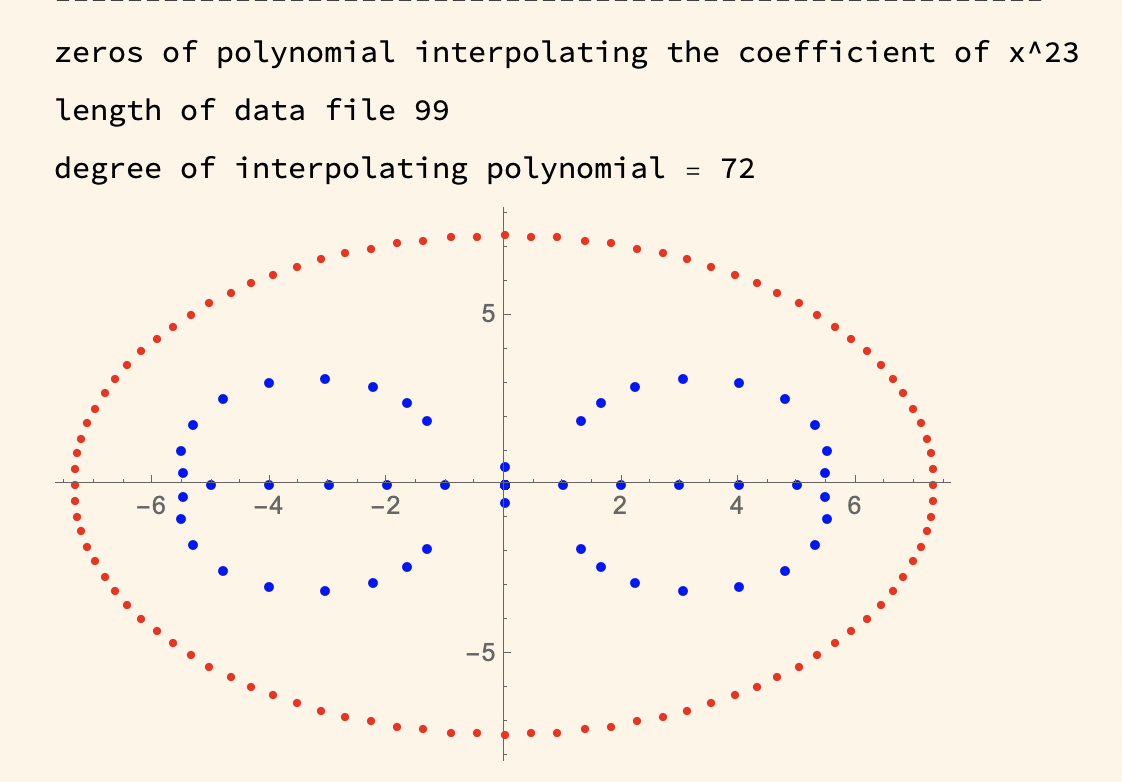
\includegraphics[scale=.7]{Figure 1.png} 
\sc{Roots of polynomial interpolating 
the coefficient of $q_m^{23}$
in the Fourier expansion of $j_m$.}
\printbibliography
\end{document}